\chapter{Overview and Background}

\section{Hardware Architecture}

Supercomputers are usually designed with the cluster architecture that consists of a set of computing nodes. In the great majority of cases, all nodes use the same hardware and the same operating system. The nodes are connected via fast interconnect to accomplish great task parallelism. Users log on to the head node via ssh. They can distribute several tasks on computing nodes. A node may look similar to any other personal computer but is far more powerful in terms of computing power.  The nodes also have access to global data storage.

\begin{figure}[htbp]
\centering
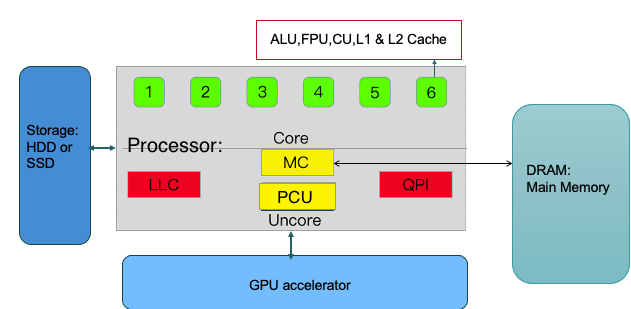
\includegraphics[width=11cm]{pictures/fig2.2}
\caption{Node}
\end{figure}

Figure 2.1 represents a computing node. It consists of processors, DRAM, local storage, and GPU accelerators. Today's microprocessors are mainly based on von Neumann architecture. The processor is divided into two areas namely core and uncore. The core consists of components that are responsible for computing and executing instructions, including control units (CU), arithmetic logic units (ALU), floating point unit (FPU),  and upper-level caches e.g. L1 and L2 cache.  The uncore contains other components that are not responsible for the computational tasks but must be closely connected to the core such as the last level cache (LLC), the memory controller (MC), the quick path interconnect (QPI) and the power control logic (PCU).  They are responsible for data communication between the processor and other components, power setting of the processor and inter-socket communication. When a program utilises core heavily, it is called compute-intensive. Instead, if a program is memory-intensive, high uncore activities will be observed. 

\subsubsection{Core}
Moore's law suggests that the number of transistors in a dense  integrated circuit doubles every one to two years \cite{39}. As a result, the clock frequency of microprocessors has grown exponentially over the last century. However, high clock frequency brings significant power consumption. Electric power brings heat dissipation problems. That is the reason that the growth rate of the clock frequency of a single core has decreased for the last few decades. If the clock frequency is too high, the cooling system of the processor cannot dissipate heat fast enough that it may damage the hardware. 

To increase the performance of the processor and limit the heat problems simultaneously, people start to focus on the development of multi-core processors. The processor showed in figure 2.1 is a 6-core processor. Each core has its own ALU, FPU, L1, and L2 cache.  Multi-core processors have huge advantages on task parallelism over single-core processors. For example, multi-core processors can break a huge task into small pieces and assign each piece to a core. Each core can operate at a lower frequency and therefore costs lower energy.
\subsubsection{Uncore}
As the core count and the size of LLC increases, the uncore occupies more on die-area \cite{17}, which contributes significant power consumption \cite{18} to the processor. The function of uncore is managing non-compute intensive workloads such as data communication between the processor and other components. The LLC is a fast but small memory located in uncore area. It stores a small amount of data that are likely to be used by the core since the core accesses the LLC much faster than the DRAM. The MC is responsible for the data communication with DRAM. The QPI allows the multiple-socket platform to communicate between sockets \cite{17}. The PCU modifies clock frequency and core voltage to coordinates the power and performance ratio \cite{17}.
\subsubsection{Memory Hierarchy}
For the last few decades, the semiconductor industry has divided microprocessors and memory into two different fields. The technology for microprocessors focused on speed while for memory on capacity. As a result, the performance improvement rate of microprocessor speed outpaced the improvement rate of memory speed \cite{10}. Figure 2.2 \cite{9} showed that the performance gap between processor and memory has been growing for the last few decades.

\begin{figure} [h] %hier können noch Positionierungswünsche angegeben werden
	\centering   % Alles weitere zentrieren
	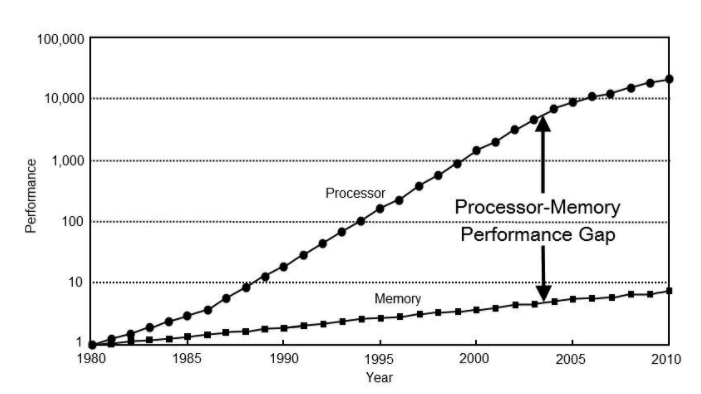
\includegraphics[width=10cm]{pictures/fig2.4}
	\caption{Performance gap between processor and memory \cite{9}}
	\label{fig1}  %Reihenfolge ist wichtig! Immer erst \caption{} dann \label{}
\end{figure}

When the processor encounters memory-intensive programs, the continuous access to the memory makes the processor wait for slower memory and stall, therefore it wastes a lot of clock cycles. In order to solve the performance gap issue, the cache is introduced. The cache is implemented as smaller size but fast accessing speed SRAM memory which located inside the processor. It is further divided into several levels. For example, Intel's processors usually have L1, L2, and L3 cache. The L1 and L2 cache are inside the core while the L3 cache is located in uncore area. The CPU is connected to different levels of memory. Figure 2.3 \cite{11} shows the abstract of the memory hierarchy. The closer the memory to the CPU, the faster but smaller it will be. When a CPU requires data, it first accesses the register directly and then followed by the cache. If the data item is not in the cache, then there is a cache miss and the processor will continue searching the main memory until the data item is found.			
	
\begin{figure} [h] %hier können noch Positionierungswünsche angegeben werden
	\centering   % Alles weitere zentrieren
	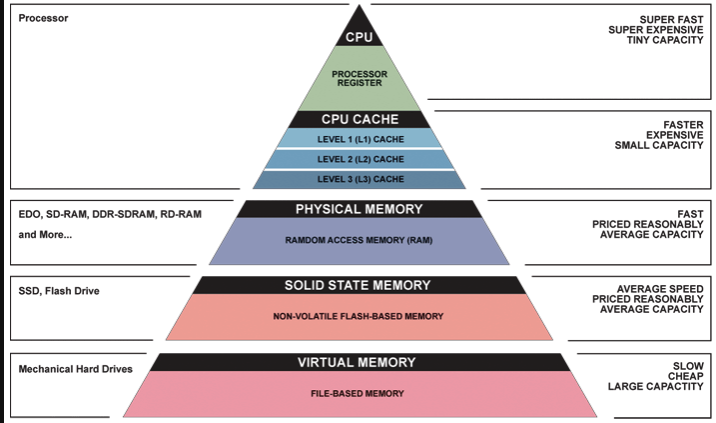
\includegraphics[width=10cm]{pictures/fig2.5}
	\caption{Memory hierarchy \cite{11}}
	\label{fig1}  %Reihenfolge ist wichtig! Immer erst \caption{} dann \label{}
\end{figure}

\subsubsection{Graphic Processing Unit}
A GPU is a specialized processor to accelerate graphics rendering. The biggest difference between a GPU and a CPU is that the GPU has thousands of sub-cores. This makes the GPU more efficient than the CPU on parallel computing. Today's supercomputers commonly use a general purpose graphics processing unit (GPGPU) which not only handles computation for computer graphics but also performance general CPU tasks. In some applications that require massive vector operations, the GPGPU is proven to be far more efficient than the CPU. In this work, the focus is on the tuning of the processor's frequency.

\section{Power Management}
The thermal design power (TDP) is the maximum power that the cooling system in a computer is needed to dissipate. It is not the maximum power a processor can consume but a power budget for the system to operate safely. For example, a processor is designed with 50W TDP, which means that the cooling system can dissipate in maximal 50W of heat without exceeding the maximum temperature for the CPU. HPCs have several functionalities to maintain a power consumption and make sure it operates safely.
\subsubsection{Running Average Power Limit}
Running Average Power Limit (RAPL) is a mechanism implemented in hardware that monitors the power consumption of CPU and DRAM \cite{19}. It was first introduced in Intel's Sandy Bridge microarchitecture. RAPL provides several counters to monitor the power and energy consumption of the processor package and DRAM over a sliding time frame. Another functionality of RAPL is to maintain a power cap of the average power consumption of the processor. Programmers can measure or constrain the power consumption of DRAM and processor package(core and uncore) by modifying the model-specific registers (MSRs) \cite{21}.
\subsubsection{Dynamic Voltage and Frequency Scaling}
DVFS \cite{22} is a widely used technique to save power on modern computers. According to Etienne Le Sueur et al., the dynamic power consumption is 
\begin{equation}
P = CfV^2
\end{equation}
where $P$ is the dynamic power, C is the capacitance and V is the voltage. When the frequency is lowered, the corresponding voltage will be reduced significantly. DVFS dynamically modifies the core frequency and the supply voltage to achieve power saving.

%\subsubsection{LIKWID}
%LIKWID is short for "like I know what I'm doing".
\subsubsection{Uncore Frequency Scaling}
Intel separates the core and uncore frequency from the Haswell microarchitecture onward. The uncore frequency scaling (UFS) is therefore introduced. Programmers can use UFS to modify the uncore frequency regardless of the core's operating state \cite{21}. This subsection analyses the impact of uncore frequency on performance using one Haswell node. The node contains one Intel(R) Xeon(R) processor E5 v3 @ 2.30GHz which has 18 cores. The node has 32GB of memory. 

Three benchmarks from the NAS parallel benchmark \cite{23} suit namely Block Tridiagonal solver (BT), Multi-grid solver (MG) and Embarrassingly Parallel (EP) are used. BT is an LLC cache-bound benchmark, MG is a memory-bound benchmark and EP is a compute-intensive benchmark. Each of them has unique performance characteristics that help to evaluate the impact of uncore frequency on performance. The openMP version of those benchmarks are  used. The uncore frequency is reduced from 3.0 GHz to 1.2 GHz in steps of 0.1 GHz. The PKG power and DRAM power in Watts,  completion time in seconds and memory bandwidth in GB/s are recorded. The experiments were repeated 3 times and the average values of the result  are presented. 

Table 2.1 presents the completion time, PKG power, DRAM power, memory bandwidth and last level cache miss per second for BT, MG and EP at default uncore frequency (3.0GHz). All of them are measured by LIKWID. Figure 2.4 (a), (b) and (c) present the performance impact of uncore frequency on those data. The x-axis is the uncore frequency while the y-axis shows all the data normalised with respect to the default uncore frequency (3.0 GHz). 

\begin{table} %[htbp] %hier können noch Positionierungswünsche angegeben werden
	\centering      % Alles weitere zentrieren
	\begin{tabular}{|c|c|c|c|} %Alle Spalten zentrieren, ansonsten 'r' oder 'l'
		\hline
		\textbf{Metric} & \textbf{BT} &\textbf{MG} & \textbf{EP}  \\
		\hline
		Completion time(s)              & 75.4  & 1.2  &    5.56        \\
		\hline
		PKG power(W)	              &  140& 119 &   129.      \\
		\hline
		DRAM power(W)		 &   11 &   16 & 5 \\
		\hline	
		Memory bandwidth(GB/s)  &  20 & 41 & 0.049\\

		\hline

		
		
		\hline
	\end{tabular}
	\caption{Performance metrics for BT, MG and EP @ 3.0 GHz}
	%\label{tab:vergleich}  %Reihenfolge ist wichtig! Immer erst \caption{} dann \label{}
\end{table}

Figure 2.4 (a) presents the performance impact of uncore frequency on the memory-bound benchmark MG. As the uncore frequency is reduced from 3 GHz to 1.4 GHz, the job completion time increases linearly. When the uncore frequency is lowered under 1.4 GHz, the completion time increases faster. It suggests that for memory-bound applications, the decrease in uncore frequency results in significant performance degradation. The reason is that the memory controllers operate slower at a lower uncore frequency \cite{21}. There will be fewer memory requests that are sent by the controllers. Therefore, the DRAM power decreases which makes the DRAM read or write data slower. 

Figure 2.4 (b) presents the results on the compute-bound benchmark EP. As the uncore frequency is reduced, the PKG power decreases significantly. In the meantime, the job completion time is not affected. There are no obvious changes on the DRAM power and memory bandwidth because EP does not utilize memory controller nor LLC\cite{21}. For compute-bound applications, the uncore frequency can be reduced to achieve power-saving without performance downgrading.

Figure 2.4 (c) presents the results on the LLC-bound benchmark BT. The DRAM power does not change during the experiment. When the uncore frequency is greater than 2.5 GHz, there are no obvious changes on each of the datasets.  As the uncore frequency is reduced from 2.5 GHz to 1.7 GHz, the package power and memory bandwidth decrease but the execution time increases slowly. When the uncore frequency is reduced under 1.7 GHz, the completion time increased aggressively. For LLC-bound applications, it is possible to reduce the uncore frequency within a certain limit. If a small-scale of performance downgrading is acceptable, the uncore frequency can be reduced sightly to save power.

From the result of Figure 2.4, the following conclusions can be drawn
\begin{enumerate}
\item Lowering the uncore frequency downgrades the memory-intensive applications
\item For compute-intensive applications the uncore frequency can be lowered without performance downgrading.
\item For LLC intensive applications the uncore frequency can be lowered up to a certain limit.
\end{enumerate}

\begin{figure}
  \centering
  \subfigure[MG]{
    \label{fig:subfig:a} %% label for first subfigure
    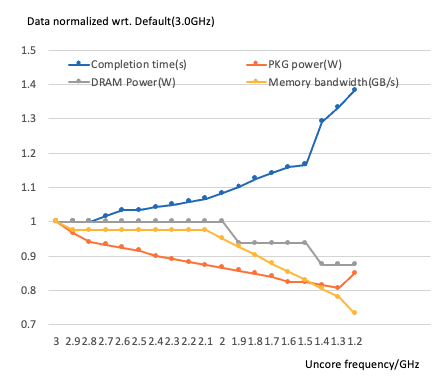
\includegraphics[width=3in]{pictures/mg}}
  \hspace{0.000001in}
  \subfigure[EP]{
    \label{fig:subfig:b} %% label for second subfigure
    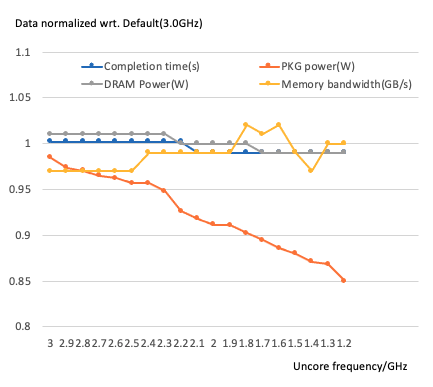
\includegraphics[width=3in]{pictures/ep}}
     \hspace{0.000001in}
  \subfigure[BT]{
    \label{fig:subfig:b} %% label for second subfigure
    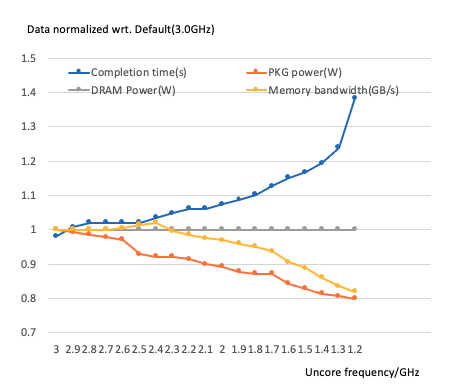
\includegraphics[width=3in]{pictures/bt}}
  \caption{Performance impact of uncore frequency on MG, EP and BT}
  \label{fig:subfig} %% label for entire figure
\end{figure}


